\documentclass[12pt, dvipdfmx]{beamer}

\renewcommand{\kanjifamilydefault}{\gtdefault}
%%%%%%%%%%%  package  %%%%%%%%%%%
\usepackage{bxdpx-beamer}% dvipdfmxなので必要
\usepackage{pxjahyper}% 日本語で'しおり'したい

\usepackage{amssymb,amsmath,ascmac}

\usepackage{multirow}
\usepackage{bm}

\graphicspath{{../../_Figures//}{../../_Figures/Rheology/}}

\usepackage{tikz}
\usepackage{xparse}

\usetikzlibrary{shapes,arrows}
%% define fancy arrow. \tikzfancyarrow[<option>]{<text>}. ex: \tikzfancyarrow[fill=red!5]{hoge}
\tikzset{arrowstyle/.style n args={2}{inner ysep=0.1ex, inner xsep=0.5em, minimum height=2em, draw=#2, fill=black!20, font=\sffamily\bfseries, single arrow, single arrow head extend=0.4em, #1,}}
\NewDocumentCommand{\tikzfancyarrow}{O{fill=black!20} O{none}  m}{
\tikz[baseline=-0.5ex]\node [arrowstyle={#1}{#2}] {#3 \mathstrut};}

%目次スライド
\AtBeginSection[]{
  \frame{\tableofcontents[currentsection]}
}

%アペンディックスのページ番号除去
\newcommand{\backupbegin}{
   \newcounter{framenumberappendix}
   \setcounter{framenumberappendix}{\value{framenumber}}
}
\newcommand{\backupend}{
   \addtocounter{framenumberappendix}{-\value{framenumber}}
   \addtocounter{framenumber}{\value{framenumberappendix}} 
}

%%%%%%%%%%%  theme  %%%%%%%%%%%
\usetheme{Copenhagen}
% \usetheme{Metropolis}
% \usetheme{CambridgeUS}
% \usetheme{Berlin}

%%%%%%%%%%%  inner theme  %%%%%%%%%%%
% \useinnertheme{default}

% %%%%%%%%%%%  outer theme  %%%%%%%%%%%
\useoutertheme{default}
% \useoutertheme{infolines}

%%%%%%%%%%%  color theme  %%%%%%%%%%%
%\usecolortheme{structure}

%%%%%%%%%%%  font theme  %%%%%%%%%%%
\usefonttheme{professionalfonts}
%\usefonttheme{default}

%%%%%%%%%%%  degree of transparency  %%%%%%%%%%%
%\setbeamercovered{transparent=30}

% \setbeamertemplate{items}[default]

%%%%%%%%%%%  numbering  %%%%%%%%%%%
% \setbeamertemplate{numbered}
\setbeamertemplate{navigation symbols}{}
\setbeamertemplate{footline}[frame number]


\title
[レオロジーのはじめの一歩]
{レオロジーのはじめの一歩}
\author[東亞合成 佐々木]{佐々木 裕\thanks{hiroshi\_sasaki@mail.toagosei.co.jp}}
\institute[東亞合成]{東亞合成株式会社}
\date{}

\begin{document}

%%%%%
% 1 P
%%%%%
\maketitle

%%%%%
% 2 P
%%%%%
%% 目次 (必要なければ省略)
\begin{frame}
\frametitle{Outline}
\tableofcontents
\end{frame}

\begin{frame}
	\frametitle{この章でのお話}
	ここでは、固体と液体という基本的な物質の有り様について、考えていきます。
		\begin{boxnote}
			\begin{itemize}
				\item 固体の最も基本的なモデルである弾性体という状態を考えます。
				\item 刺激と応答を表すために、ひずみと応力を使うことで力学モデルが書けることを学びます。
				\item つづいて、液体が流れるということを考えます。
				\item 液体の力学モデルが、「ひずみ速度」で表されることを学びます。
			\end{itemize} 
		\end{boxnote}
\end{frame}

\section{レオロジーのはじめの⼀歩}
\subsection{レオロジーのやり方の再確認}
\begin{frame}
	\frametitle{レオロジーのやり方の再確認}
	\begin{block}{レオロジーのやり方}
		レオロジーとは物質に刺激を与えてその応答を評価観察することで、その特性を評価できるのでした。\\
	ここでは、わかり易い例として、物質の力学的なレオロジー評価を考えてみましょう。
	\end{block}
	\begin{columns}[T, onlytextwidth]
		\column{.58\linewidth}
			\includegraphics[width=\textwidth]{Rheo_method.png}
		\column{.38\linewidth}
			\begin{itemize}
				\item 力学的な刺激
				\begin{itemize}
					\item 外力による\\物質の変形
				\end{itemize}
				\item 変形の結果として
				\begin{itemize}
					\item 応力が発生
					\item 流動が生じる\\場合も。
				\end{itemize}
			\end{itemize}
	\end{columns}
\end{frame}

\subsection{力について}
\begin{frame}
	\frametitle{力とは}
		\begin{block}{「力」とは}
			{\large 「物体の状態を変化させる原因となる作用で、\\その作用の大きさを表す物理量」}
		\end{block}	
		\begin{exampleblock}{「状態の変化」に関して二通り}
			\begin{itemize}
				\alert<2>{
				\item 静力学
				\begin{itemize}
					\item 静的状態(時間によって系の位置が変化しない状態)に働く力に関して、
					\item 主として、\alert{力の釣り合い}を議論。
				\end{itemize}
				}
				\item 動力学
				\begin{itemize}
					\item 運動量の変化を伴う質点の移動について議論し、
					\item \alert{相互作用する物体系の運動}について議論。
				\end{itemize}
			\end{itemize}
		\end{exampleblock}
\end{frame}

\subsection{物質の変形と仕事}
\begin{frame}
	\frametitle{物質の変形と仕事}
		\begin{block}{静的な釣り合いとしての力}
			\begin{itemize}
				\item 物質の外から加えた力を外力として、
				\item 物質の内部に、外力に抵抗する力として内力が生じ、
				\item 外力と内力が釣り合う。$\Leftrightarrow$ 「作用・反作用の原理」
			\end{itemize}
		\end{block}
		\begin{alertblock}{外力に対応して物質は変形}
			\begin{itemize}
				\item 釣り合いのもとでの\alert{物質の変形も、仕事}となる。
				\item この場合、外力が物質の内部に蓄積された(弾性)エネルギーに相当する量の仕事を行ったと考える。
				\item この事の詳細は、また後ほど。
			\end{itemize}
		\end{alertblock}
\end{frame}

\section{弾性体の力学的な刺激と応答}
\subsection{弾性体の力学的な刺激と応答}
\begin{frame}
	\frametitle{弾性体の力学的な刺激と応答}
		\begin{exampleblock}{弾性体とは:}
			\begin{itemize}
				\item 最も簡単な固体のモデル
				\item 変形を受けても
				\begin{itemize}
					\item その起源となる外力を除去すれば、
					\item 全く元の状態に戻るような性質
				\end{itemize}
			\end{itemize}
		\end{exampleblock}		
		\begin{block}{弾性体の力学的な刺激と応答}
			\begin{itemize}
				\item 外力による物質の変形
				\begin{itemize}
					\item 引張変形
					\item せん断変形
				\end{itemize}
				\item 変形の結果として
				\begin{itemize}
					\item 物質はひずむ
					\item 内部で応力が発生
				\end{itemize}
			\end{itemize}
		\end{block}
\end{frame}

\subsection{変形とひずみ}
\begin{frame}
	\frametitle{二つの変形とひずみ}
	外力と加えたときに弾性体に生じる変形を、\\以下の二つに単純化
	\begin{itemize}
		\item 物質を一つの軸に沿って引き伸ばす「引張変形」
		\item トランプのカードを横にずらしたような「せん断変形」
	\end{itemize}
	\begin{columns}[c, onlytextwidth]
		\column{.4\linewidth}
			\begin{center}
				\includegraphics[width=0.9\textwidth]{Causy.png}
				「引張変形」
			\end{center}
		\column{.4\linewidth}
			\begin{center}
				\includegraphics[width=0.9\textwidth]{Shear.png}
				「せん断変形」
			\end{center}
	\end{columns}
\end{frame}

\begin{frame}
	\frametitle{引張変形とコーシーひずみ}
	引張変形による物質のひずみを記述する最も単純なものが、\\
	「コーシーひずみ」 \\(一般に、伸長ひずみはギリシア文字の $\varepsilon$) 
	\begin{columns}[c, onlytextwidth]
		\column{.4\linewidth}
			% \textbf{コーシーひずみ:}
			\begin{align*}
				\varepsilon_c &= \dfrac{\text{\textbf{変形量}}}{\text{\textbf{変形前の長さ}}} \\
				&=\dfrac{\Delta L}{L_0} = \dfrac{L-L_0}{L_0}
			\end{align*}
		\column{.59\linewidth}
			\begin{center}
				\includegraphics[width=0.6\textwidth]{Causy.png}
			\end{center}
	\end{columns}
	\vspace{3mm}
	「ひずみは、長さを長さで割っているので、次元を持たない無次元量」
\end{frame}

\begin{frame}
	\frametitle{せん断変形とせん断ひずみ}
	せん断変形によるひずみは、\\ (せん断ひずみはギリシア文字の $\gamma$) 
	\begin{columns}[c, onlytextwidth]
		\column{.4\linewidth}
			% \textbf{せん断ひずみ:}
			\begin{itemize}
				\item 高さ $h$ を一定
				\item 横に $x$ 変形
			\end{itemize}
			\begin{align*}
				\gamma &= \dfrac{\text{\textbf{変形方向への変形量}}}{\text{\textbf{サンプルの厚み}}} \\
				&=\dfrac{x}{h}
			\end{align*}
		\column{.59\linewidth}
			\begin{center}
				\includegraphics[width=0.9\textwidth]{Shear.png}
			\end{center}
	\end{columns}
	\vspace{3mm}
	「ひずみは、長さを長さで割っているので、次元を持たない無次元量」
\end{frame}

\subsection{応力について}
\begin{frame}
	\frametitle{応力のイメージ}
	\begin{exampleblock}{応力とは、}
		\begin{itemize}
			\item 物質の内部に生じている力の大きさを表す物理量
			\item 単位面積あたりに働く内部の力
		\end{itemize}
		棒の長手方向にはどの位置で切断したとしても、\\ \alert{同一の応力が働いている}ことに注意
	\end{exampleblock}
	\begin{columns}[T, onlytextwidth]
		\column{.25\linewidth}
			\begin{align*}
				[\text{応力}] &= \dfrac{[\text{力}]}{[\text{面積}]} \\
					&= \dfrac{[N]}{[m]^2} \\
					&= [\mathrm{Pa}]
			\end{align*}
		\column{.7\linewidth}
			\begin{center}
				\includegraphics[width=\textwidth]{Stress.png}
				% 引張変形を与えた場合の外力と応力のイメージ
			\end{center}
	\end{columns}
\end{frame}

\begin{frame}
	\frametitle{伸長応力$\sigma$}
	伸長時に働く応力は、一般に、ギリシア文字の $\sigma$ と表記
	\begin{columns}[T, onlytextwidth]
		\column{.48\linewidth}
		\begin{align*}
			\sigma = &= \dfrac{\text{\textbf{与えた力}}}{\text{\textbf{断面積}}} \\
				&=\dfrac{F}{A} [\mathrm{Pa}]
		\end{align*}
		\vspace{-3mm}
		\begin{itemize}
			\item $F$ は外部からの外力
			\item $A$ は内部の断面積
		\end{itemize}
		\begin{alertblock}{同一の外力でも}
			\begin{itemize}
				\item 断面積が小さくなれば、
				\item 反比例して応力は増加
			\end{itemize}
		\end{alertblock}
		\column{.48\linewidth}
			\begin{center}
				\includegraphics[width=.8\textwidth]{elong_stress.png}
			\end{center}
	\end{columns}
\end{frame}

\begin{frame}
	\frametitle{せん断応力$\tau$}
	\begin{itemize}
		\item 互いに向かい合う同じ大きさの力である\alert{偶力 $\mathrm{F}$} を作用
		% \item せん断変形を生じた場合のせん断応力
		\item せん断の場合は、応力を $\tau$ と表記
	\end{itemize}
	\begin{columns}[T, onlytextwidth]
		\column{.48\linewidth}
			\begin{align*}
				\tau &= \dfrac{\text{\textbf{与えた力}}}{\text{\textbf{働かせた面積}}} \\
				&= \dfrac{F}{A} [\mathrm{Pa}]
			\end{align*}
			\alert{力を働かせた上面の面積が $A$ であることに注意}
		\column{.48\linewidth}
			\begin{center}
				\includegraphics[width=\textwidth]{shear_2.png}
			\end{center}
	\end{columns}
\end{frame}

\begin{frame}
	\frametitle{せん断応力のイメージ}
		\begin{itemize}
			\item サンプルの厚さ方向には、
			\begin{itemize}
				\item どの位置であっても\alert{同一のせん断応力}が作用
				\item どの位置で切断したとしても同一の偶力が作用
			\end{itemize}
			\item トランプのカードが重なったデッキを想像
			\begin{itemize}
				\item デッキの間に挟まったカードは、
				\item 一枚上のカードと下のカードによって応力を受ける
			\end{itemize}
		\end{itemize}
		\begin{center}
			\includegraphics[width=\textwidth]{trump_deck.png}
		\end{center}
\end{frame}

\section{力学モデルについて}
\subsection{弾性体の力学モデル}
\begin{frame}
	\frametitle{弾性体の力学モデル}
	ここまで刺激と応答の例として使ってきた弾性体を、物質として評価する方法について考えてみましょう。
	\begin{exampleblock}{ここで目指すこと}
		\begin{itemize}
			\item 弾性体の力学的な応答を、イメージしたい。
			\begin{itemize}
				\item 分かりやすいアナロジーでイメージする。
				\item 絵として理解したい。
			\end{itemize}
			\item 異なる物質を定量的に評価したい。
			\begin{itemize}
				\item 共通な性質を見出す。
				\item 力学的な応答を数式として力学モデルとする。
			\end{itemize}
		\end{itemize}
	\end{exampleblock}
	弾性体の力学応答を書き表すことが出来る力学モデルを\\数式として表すことで、\alert{「異なる物質を定量的に比較」}\\できるようになることを目指すわけです。
\end{frame}

\begin{frame}
	\frametitle{バネの力学的な振る舞いを表すフックの法則}
		\begin{screen}
			\begin{itemize}
				\item これまでの経験から、弾性体はバネのように取り扱えることが知られています。
				\item バネの力学的な振る舞いには、イギリスの物理学者 Robert Hooke が見出した「フックの法則」と呼ばれる以下の関係があることがわかっています。
			\end{itemize}
		\end{screen}
		\begin{columns}[c, onlytextwidth]
			\column{.48\linewidth}
				\begin{block}{「フックの法則」}
					\begin{itemize}
						\item バネの伸びと力は比例
					\end{itemize}
					\vspace{-1mm}
					\begin{align*}
						\text{力} &= \text{比例定数} \times \text{変位量} \\
						F(x) &= k x
					\end{align*}
				\end{block}
			\column{.48\linewidth}
				\begin{center}
					\includegraphics[width=.9\textwidth]{spring.png}
				\end{center}
		\end{columns}
\end{frame}

\begin{frame}
	\frametitle{弾性体の力学モデル}
		伸長変形の力学モデルは、フックの法則に従う形で、
	\begin{columns}[c, onlytextwidth]
		\column{.52\linewidth}
			\begin{block}{伸張変形の力学モデル}
				\begin{itemize}
					\item 変形ひずみ $\varepsilon$ と比例して、
					\item 伸長応力 $\sigma$ が生じ、
					\item 比例定数が引張弾性率 $E$
				\end{itemize}
				\begin{align*}
					\sigma = E \varepsilon 
				\end{align*}
			\end{block}
		\column{.46\linewidth}
		\begin{center}
			\includegraphics[width=\textwidth]{hook_law.png}
		\end{center}
	\end{columns}
	\begin{screen}
		\begin{itemize}
			\item ひずみは無次元量なので、
			\item 引張弾性率 $E$ は伸長応力 $\sigma$ と同じ組立単位 $[\mathrm{Pa}]$
		\end{itemize}
	\end{screen}
\end{frame}

\begin{frame}
	\frametitle{せん断変形の力学モデル}
	% フックモデルは、せん断変形の場合にも適応できる。
		\begin{block}{せん断変形の力学モデル}
			\vspace{-3mm}
			\begin{align*}
				\text{せん断応力} &= \text{せん断弾性率} \times \text{せん断ひずみ} \\
				\tau &= G \gamma
			\end{align*}
			比例定数は、せん断弾性率と呼ばれ、$G[Pa]$
		\end{block}
			\begin{center}
				\includegraphics[width=\textwidth]{trump_deck.png}
			\end{center}
\end{frame}

\subsection{液体の変形と応答}
\begin{frame}
	\frametitle{流れるという性質}
	液体は、変形されたら元には戻れない $\Leftrightarrow$ \alert{「流れる」}
	\begin{block}{流れるという性質}
		\begin{columns}[T, onlytextwidth]
			\column{.65\linewidth}	
				\begin{itemize}
					\item コップの中ではじっとしている。
					\item 変形を与えると流れる
						\begin{itemize}
							\item \alert{元には戻らない。}
							\item 変形を止めれば、応力も消失
						\end{itemize}
					\item 応答を見るのが困難
						\begin{itemize}
							\item \alert{変形を続けながら応力を測る}
							\item 液体内部の変形と応力を見積る
						\end{itemize}
					\item 液体の評価
						\begin{itemize}
							\item その形状を維持しやすい\\「せん断変形」
							% \item 測定の間、せん断変形を\\与え続ける
						\end{itemize}
				\end{itemize}
			\column{.3\linewidth}
				\vspace{-3mm}
				\begin{center}
					\includegraphics[width=.8\textwidth]{cup_water.png}
					\includegraphics[width=\textwidth]{river_00002.jpg}
				\end{center}
		\end{columns}
	\end{block}
\end{frame}

\begin{frame}
	\frametitle{液体の性質を直感的に理解}
		\begin{columns}[T, onlytextwidth]
			\column{.25\linewidth}
					\begin{center}
						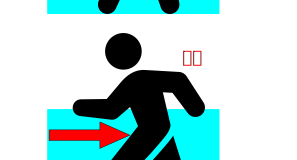
\includegraphics[width=\textwidth]{pool_walking.png}
					\end{center}
			\column{.7\linewidth}
				\begin{block}{プールでの水中歩行の例}
					液体が生じる力を直感的に理解するために、プールでの水中歩行を考えてみます。
					\begin{itemize}
						\item ゆっくりと歩いて移動(上の図)
						\begin{itemize}
							\item 受ける抵抗はそれほど大きくない。
						\end{itemize}
						\item 走って速く移動(下の図)
						\begin{itemize}
							\item 速く歩こうとすると、とたんに水の抵抗は大きくなります。
						\end{itemize}
					\end{itemize}
				\end{block}
				\begin{exampleblock}{液体の性質}
					\alert{変形させる速度}が変わると、生じる力も変わる。
				\end{exampleblock}
		\end{columns}
\end{frame}

\subsection{液体の力学モデル}
\begin{frame}
	\frametitle{ニュートンの法則}
	古典力学の土台を築いたニュートンが以下を導出。
	\begin{columns}[c, onlytextwidth]
		\column{.66\linewidth}
		\begin{itemize}
			\item 流れの\alert{せん断応力 $\tau$ }と
			\item その\alert{せん断速度 $\dot{\gamma}$ }との間に
			\item \alert{比例関係}を見出している
			\item 右図の円筒形の測定装置で、\\
			% 以下のパラメタを変化
			\begin{itemize}
				\item 液厚 $h$ 
				\item 回転速度 $v$
			\end{itemize}
		\end{itemize}
		\column{.32\linewidth}
			\begin{center}
				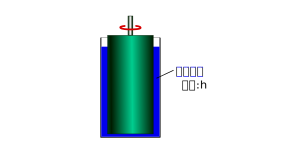
\includegraphics[width=.9\textwidth]{nijyu_entou.png}
			\end{center}
	\end{columns}
	\begin{exampleblock}{ニュートンの法則}
		\vspace{-5mm}
		\begin{align*}
			\text{せん断応力} &= \text{比例定数} \times \text{せん断速度} \notag \\
			\tau = \eta \dot{\gamma}
		\end{align*}
		% \vspace{-4mm}
		\alert{比例定数が、物質の流れ易さを表す「粘度」 $\eta$}
		% \vspace{-2mm}
		% \begin{align*}
		% 	[\text{粘度}] = \dfrac{[\text{せん断応力}]}{[\text{せん断速度}]} 
		% 	= \dfrac{[\mathrm{Pa}]}{[\mathrm{s^{-1}}]} = [\mathrm{Pa\cdot s}]
		% \end{align*}
	\end{exampleblock}
\end{frame}

\begin{frame}
    \frametitle{ニュートンの法則}
		\begin{columns}[T, onlytextwidth]
			\column{.48\linewidth}
				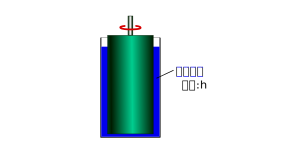
\includegraphics[width=.7\textwidth]{nijyu_entou.png}
			\column{.48\linewidth}
				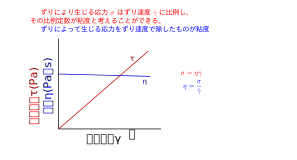
\includegraphics[width=.9\textwidth]{newtonian.png}
		\end{columns}
		\begin{exampleblock}{ニュートンの法則}
			\vspace{-5mm}
			\begin{align*}
				\text{せん断応力} &= \text{比例定数} \times \text{せん断速度} \notag \\
				\tau = \eta \dot{\gamma}
			\end{align*}
			% \vspace{-4mm}
			\alert{比例定数が、物質の流れ易さを表す「粘度」 $\eta$}
		\end{exampleblock}
\end{frame}

\begin{frame}
	\frametitle{液体の力学モデル}
		\begin{columns}[T, onlytextwidth]
			\column{.48\linewidth}
				\begin{exampleblock}{液体のモデル}
					\begin{itemize}
						\item 液体の振る舞いを表すモデル
						\item 右図のダッシュポット
						\item イメージとしては、\\水鉄砲
						\item 速くピストンを動かすと、抵抗が大。
					\end{itemize}
				\end{exampleblock}
			\column{.48\linewidth}
				\includegraphics[width=\textwidth]{dashpot.png}
		\end{columns}
\end{frame}

\begin{frame}
	\frametitle{力学モデルのまとめ}
			\begin{center}
				\begin{tabular}{|c||c|} \hline
					固体のモデル	& 液体のモデル \\ \hline \hline
					応力は\alert{ひずみに比例}	& 応力は\alert{ひずみ速度に比例}\\
					$\text{応力} = \text{弾性率} \times \text{ひずみ}$	& $\text{応力} = \text{粘度} \times \text{ひずみ速度}$ \\ \hline
					比例定数が弾性率	& 比例定数が粘度\\ 
					弾性率の単位は、[Pa]	& 粘度の単位は、[Pa$\cdot$s]\\ \hline
					\includegraphics[width= 0.3\textwidth]{spring.png} & \includegraphics[width=.3\textwidth]{dashpot.png} \\ \hline
				\end{tabular}
			\end{center}
\end{frame}

% \section{この章のまとめ}
\begin{frame}
	\frametitle{まとめ}
	この章では、固体と液体という基本的な物質のふるまいを書き表す一番単純なモデルについて、説明を進めました。
	\begin{boxnote}
			\begin{itemize}
				\item 刺激と応答を表すために、「ひずみと応力」を使うことで力学モデルが書けること
				\item 固体の力学モデルが、「ひずみ」に比例すること
				\item 液体の力学モデルが、「ひずみ速度」で表されること
			\end{itemize} 
	\end{boxnote}
\end{frame}

% \appendix
% \backupbegin

% \section{演習問題 1}
% \subsection{「弾性体の力学的な刺激と応答」}
% \begin{frame}
% 	\frametitle{「弾性体の力学的な刺激と応答」}
% 	\small
% 	% 以下の穴を埋めてください。
% 	\begin{itemize}
% 		\item \textcolor<2>{black}{物質}に\fbox{\textcolor<1>{white}{力学的な刺激}}を与えるということは、\fbox{\textcolor<1>{white}{外力によって物質を変形}}させるということに対応します。
% 		\item このとき、変形の結果として「\fbox{\textcolor<1>{white}{物質の内部で応力}}」という応答が生じます。
% 		\item 変形は、物質を一つの軸に沿って引き伸ばす「\fbox{\textcolor<1>{white}{引張変形}}」とトランプのカードを横にずらしたような「\fbox{\textcolor<1>{white}{せん断変形}}」の二つに単純化できます。
% 		\item \fbox{\textcolor<1>{white}{変形量}}を\fbox{\textcolor<1>{white}{変形前の長さ}}で除したものがみとなります。
% 	\end{itemize}
% \end{frame}

% \begin{frame}
% 	\frametitle{「弾性体の力学的な刺激と応答」}
% 	\small
% 	% 以下の穴を埋めてください。
% 	\begin{itemize}
% 		\item \textcolor<2>{black}{応力}とは、\fbox{\textcolor<1>{white}{物質の内部に生じている力の大きさ}}を表す物理量であり、その表す意味は\fbox{\textcolor<1>{white}{単位面積あたりに働く内部の力}}ということになります。
% 		\item この関係は以下のように書けます。
% 		\begin{align*}
% 			\fbox{\textcolor<1>{white}{応力}} = \dfrac{\fbox{\textcolor<1>{white}{物体に加えた外力}}}{\fbox{\textcolor<1>{white}{内部で応力が働く断面積}}}
% 		\end{align*}
% 		\item 一様な太さの棒を引っ張ったとき、棒の長手方向にはどの位置で切断したとしても、\fbox{\textcolor<1>{white}{同一の応力}}が働いていることに注意してください。
% 	\end{itemize}
% \end{frame}

% \subsection{「弾性体の力学モデル」}
% \begin{frame}
% 	\frametitle{「弾性体の力学モデル」}
% 	\small
% 	% 以下の穴を埋めてください。
% 	\begin{itemize}
% 		\item \textcolor<2>{black}{弾性体}とは、変形を受けてもその起源となる\fbox{\textcolor<1>{white}{外力}}を除去すれば、全く\fbox{\textcolor<1>{white}{元の状態}}に戻るような性質を持つ物質です。
% 		\item 弾性体はあたかも\fbox{\textcolor<1>{white}{バネ}}のように取り扱うことができることが知られています。
% 		% \item 弾性体を表すモデルはフックの法則であり、以下のように書けます。
% 		% \begin{figure}[htb]
% 		% 	\begin{center}
% 		% 		\begin{minipage}{0.45\textwidth}
% 		% 			\begin{itemize}
% 		% 				\item \fbox{\textcolor<1>{white}{変形ひずみ}} $\varepsilon$ と比例して、
% 		% 				\item \fbox{\textcolor<1>{white}{応力}} $\sigma$ が生じ、
% 		% 				\item 比例定数が\fbox{\textcolor<1>{white}{引張弾性率}} $E$
% 		% 			\end{itemize}
% 		% 			% \begin{align*}
% 		% 			% 	\sigma = E \varepsilon
% 		% 			% \end{align*}
% 		% 		\end{minipage}
% 		% 		\begin{minipage}{0.35\textwidth}
% 		% 			\begin{center}
% 		% 			\includegraphics[width=.8\textwidth]{hook_law.png}
% 		% 			\end{center}
% 		% 		\end{minipage}
% 		% 	\end{center}
% 		% \end{figure}
% 		% \item 弾性体のフックモデルでは全体のひずみに比例するのは\fbox{\textcolor<1>{white}{応力}}であるということに注意してください。
% 	\end{itemize}
% \end{frame}

% \begin{frame}
% 	\frametitle{「弾性体の力学モデル」}
% 	\small
% 	% 以下の穴を埋めてください。
% 	\begin{itemize}
% 		% \item 弾性体とは、変形を受けてもその起源となる\fbox{\textcolor<1>{white}{外力}}を除去すれば、全く\fbox{\textcolor<1>{white}{元の状態}}に戻るような性質を持つ物質です。
% 		% \item 弾性体はあたかも\fbox{\textcolor<1>{white}{バネ}}のように取り扱うことができることが知られています。
% 		\item \textcolor<2>{black}{弾性体}を表すモデルはフックの法則であり、以下のように書けます。
% 		% \begin{figure}[htb]
% 			\begin{center}
% 				\begin{minipage}{0.45\textwidth}
% 					\small
% 					\begin{itemize}
% 						\item \fbox{\textcolor<1>{white}{変形ひずみ}} $\varepsilon$ と比例して、
% 						\item \fbox{\textcolor<1>{white}{応力}} $\sigma$ が生じ、
% 						\item 比例定数が\fbox{\textcolor<1>{white}{引張弾性率}} $E$
% 					\end{itemize}
% 					% \begin{align*}
% 					% 	\sigma = E \varepsilon
% 					% \end{align*}
% 				\end{minipage}
% 				\begin{minipage}{0.35\textwidth}
% 					\begin{center}
% 					\includegraphics[width=.8\textwidth]{hook_law.png}
% 					\end{center}
% 				\end{minipage}
% 			\end{center}
% 		% \end{figure}
% 		\item 弾性体のフックモデルでは全体のひずみに比例するのは\fbox{\textcolor<1>{white}{応力}}であるということに注意してください。
% 	\end{itemize}
% \end{frame}

% \subsection{「液体の変形と応答」}
% \begin{frame}
% 	\frametitle{「液体の変形と応答」}
% 	\small
% 	% 以下の穴を埋めてください。
% 	\begin{itemize}
% 		\item \textcolor<2>{black}{液体}は、外力によって変形されたら元には戻れない「\fbox{\textcolor<1>{white}{流れる}}」という性質を持った物質と考えることが出来る。
% 			\begin{itemize}
% 				\item 変形を与えると\fbox{\textcolor<1>{white}{流れる}}。
% 				\item 変形を止めれば、\fbox{\textcolor<1>{white}{応力}}も\fbox{\textcolor<1>{white}{消失}}。
% 				\item 変形を続けながら\fbox{\textcolor<1>{white}{応力}}を\fbox{\textcolor<1>{white}{測る}}。
% 			\end{itemize}
% 		\item 液体の評価は主としてその\fbox{\textcolor<1>{white}{形状}}を維持しやすい「\fbox{\textcolor<1>{white}{せん断変形}}」により行われる場合が多くなります。
% 		% \item この比例関係を式で表せば以下のようになります。
% 		% 	\begin{align*}
% 		% 		\text{\fbox{\textcolor<1>{white}{せん断応力}}} &= \text{\fbox{\textcolor<1>{white}{比例定数}}} \times \text{\fbox{\textcolor<1>{white}{せん断速度}}} \notag \\
% 		% 		\tau &= \eta \dot{\gamma}
% 		% 	\end{align*}
% 		% \item 式中で示した比例定数が、物質の\fbox{\textcolor<1>{white}{流れ易さ}}を表す指標である「\fbox{\textcolor<1>{white}{粘度}}」となります。
% 	\end{itemize}
% \end{frame}

% \begin{frame}
% 	\frametitle{「液体の変形と応答」}
% 	\small
% 	% 以下の穴を埋めてください。
% 	\begin{itemize}
% 		% \item \textcolor<2>{black}{液体}は、外力によって変形されたら元には戻れない「\fbox{\textcolor<1>{white}{流れる}}」という性質を持った物質と考えることが出来る。
% 		% 	\begin{itemize}
% 		% 		\item 変形を与えると\fbox{\textcolor<1>{white}{流れる}}。
% 		% 		\item 変形を止めれば、\fbox{\textcolor<1>{white}{応力}}も\fbox{\textcolor<1>{white}{消失}}。
% 		% 		\item 変形を続けながら\fbox{\textcolor<1>{white}{応力}}を\fbox{\textcolor<1>{white}{測る}}。
% 		% 	\end{itemize}
% 		% \item 液体の評価は主としてその\fbox{\textcolor<1>{white}{形状}}を維持しやすい「\fbox{\textcolor<1>{white}{せん断変形}}」により行われる場合が多くなります。
% 		\item \textcolor<2>{black}{この}比例関係を式で表せば以下のようになります。
% 			\begin{align*}
% 				\text{\fbox{\textcolor<1>{white}{せん断応力}}} &= \text{\fbox{\textcolor<1>{white}{比例定数}}} \times \text{\fbox{\textcolor<1>{white}{せん断速度}}} \notag \\
% 				\tau &= \eta \dot{\gamma}
% 			\end{align*}
% 		\item 式中で示した比例定数が、物質の\fbox{\textcolor<1>{white}{流れ易さ}}を表す指標である「\fbox{\textcolor<1>{white}{粘度}}」となります。
% 	\end{itemize}
% \end{frame}

% \backupend

\end{document}